\documentclass[tikz,border=0pt]{standalone}
\usepackage{fontspec}
\IfFontExistsTF{TeX Gyre Heros}{\setmainfont{TeX Gyre Heros}}{\setmainfont{Latin Modern Sans}}
\usepackage{amsmath,amssymb,booktabs,array}
\DeclareMathSizes{9}{9}{8.6}{8.6}
\usepackage{pgfplots}
\pgfplotsset{compat=1.17}
\usetikzlibrary{arrows.meta,positioning,calc,fit,shapes.geometric,backgrounds}
\definecolor{ink}{HTML}{183247}
\definecolor{blue}{HTML}{286B91}
\definecolor{teal}{HTML}{19796F}
\definecolor{orange}{HTML}{AC671F}
\definecolor{muted}{HTML}{596C78}
\tikzset{
  every node/.style={font=\fontsize{9}{11}\selectfont,text=ink},
  arr/.style={-{Stealth[length=1.7mm]},line width=.55pt,draw=muted},
  panel/.style={draw=muted!35,line width=.5pt,rounded corners=1mm,fill=white},
  box/.style={draw=blue!70,line width=.55pt,rounded corners=.8mm,fill=blue!5,align=center,inner sep=2mm},
  label/.style={font=\fontsize{9}{11}\selectfont,align=left,inner sep=0},
  paneltitle/.style={font=\bfseries\fontsize{9.5}{12}\selectfont,anchor=west,inner sep=0}
}

\begin{document}
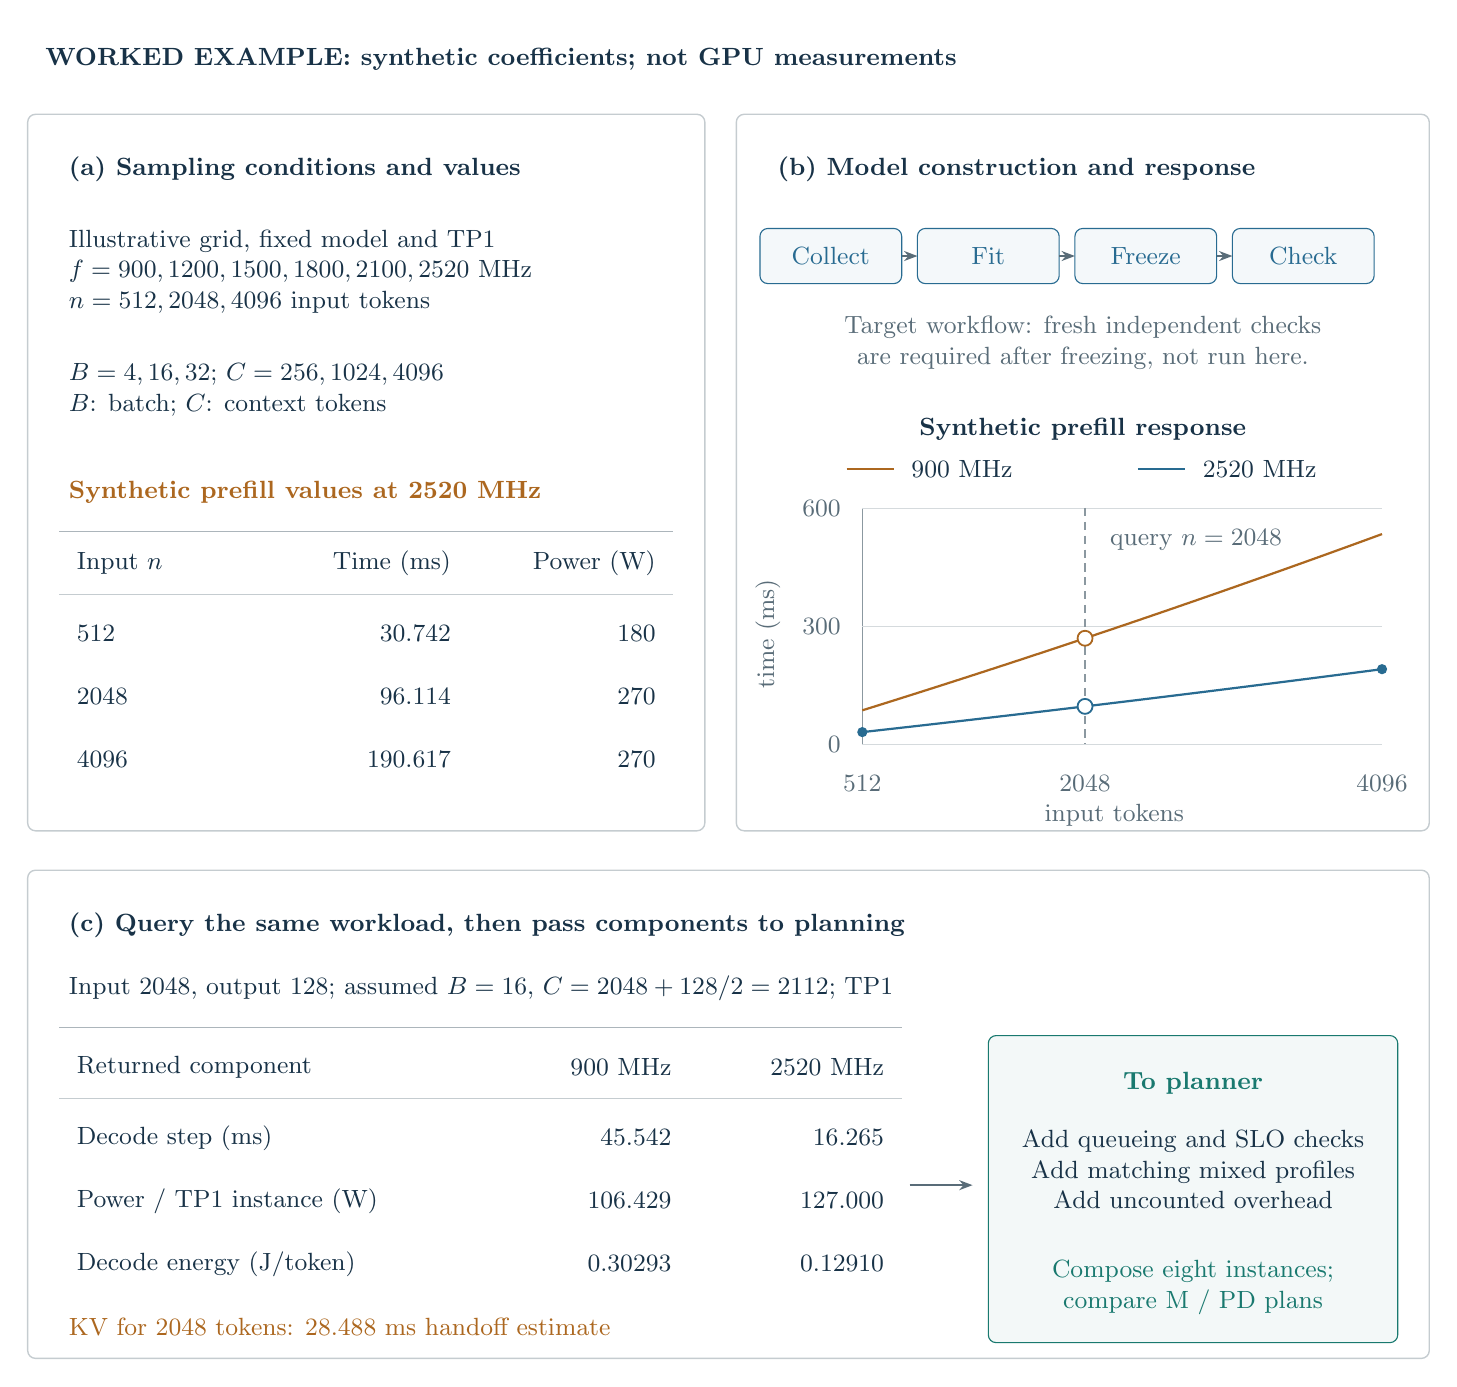
\begin{tikzpicture}[x=1mm,y=-1mm,font=\fontsize{9}{11}\selectfont]
  \path[use as bounding box] (0,0) rectangle (178,169);
  \node[anchor=west,text=ink,font=\fontsize{9}{11}\selectfont\bfseries] at (1,4)
    {WORKED EXAMPLE: synthetic coefficients; not GPU measurements};

  % Panels (a) and (b): method conditions and directly computed responses.
  \draw[panel] (0,11) rectangle (86,102);
  \draw[panel] (90,11) rectangle (178,102);
  \node[anchor=west,text=ink,font=\fontsize{9}{11}\selectfont\bfseries] at (4,18)
    {(a) Sampling conditions and values};
  \node[anchor=west,text=ink,align=left] at (4,31)
    {Illustrative grid, fixed model and TP1\\
     $f=900,1200,1500,1800,2100,2520$ MHz\\
     $n=512,2048,4096$ input tokens};
  \node[anchor=west,text=ink,align=left] at (4,46)
    {$B=4,16,32$; $C=256,1024,4096$\\
     $B$: batch; $C$: context tokens};
  \node[anchor=west,text=orange,font=\fontsize{9}{11}\selectfont\bfseries] at (4,59)
    {Synthetic prefill values at 2520 MHz};
  \draw[muted!50] (4,64) -- (82,64);
  \node[anchor=west,text=ink] at (5,68) {Input $n$};
  \node[anchor=east,text=ink] at (55,68) {Time (ms)};
  \node[anchor=east,text=ink] at (81,68) {Power (W)};
  \draw[muted!35] (4,72) -- (82,72);
  \node[anchor=west,text=ink] at (5,77) {512};
  \node[anchor=east,text=ink] at (55,77) {30.742};
  \node[anchor=east,text=ink] at (81,77) {180};
  \node[anchor=west,text=ink] at (5,85) {2048};
  \node[anchor=east,text=ink] at (55,85) {96.114};
  \node[anchor=east,text=ink] at (81,85) {270};
  \node[anchor=west,text=ink] at (5,93) {4096};
  \node[anchor=east,text=ink] at (55,93) {190.617};
  \node[anchor=east,text=ink] at (81,93) {270};

  \node[anchor=west,text=ink,font=\fontsize{9}{11}\selectfont\bfseries] at (94,18)
    {(b) Model construction and response};
  \foreach \x/\label in {102/Collect,122/Fit,142/Freeze,162/Check} {
    \node[draw=blue,rounded corners=1mm,fill=blue!5,
      minimum width=18mm,minimum height=7mm,text=blue] at (\x,29) {\label};
  }
  \draw[arr] (111,29) -- (113,29);
  \draw[arr] (131,29) -- (133,29);
  \draw[arr] (151,29) -- (153,29);
  \node[text=muted,align=center] at (134,40)
    {Target workflow: fresh independent checks\\
     are required after freezing, not run here.};
  \node[text=ink,font=\fontsize{9}{11}\selectfont\bfseries] at (134,51)
    {Synthetic prefill response};
  \draw[orange,line width=0.65pt] (104,56) -- (110,56);
  \node[anchor=west,text=ink] at (111,56) {900 MHz};
  \draw[blue,line width=0.65pt] (141,56) -- (147,56);
  \node[anchor=west,text=ink] at (148,56) {2520 MHz};

  % A hand-drawn vector plot avoids rasterization and keeps labels at 9 pt.
  % The formula is precisely synthetic_model().prefill_seconds(n, f).
  \draw[muted!70,line width=0.45pt] (106,61) -- (106,91) -- (172,91);
  \foreach \v in {0,300,600} {
    \pgfmathsetmacro{\yy}{91-\v/20}
    \draw[muted!25,line width=0.35pt] (106,\yy) -- (172,\yy);
    \node[anchor=east,text=muted] at (104.5,\yy) {\v};
  }
  \node[text=muted,rotate=90] at (94,77) {time (ms)};
  % One query position is shared by both frequency responses.
  \draw[muted!70,densely dashed,line width=0.45pt] (134.2857,61) -- (134.2857,91);
  \draw[orange,line width=0.8pt,smooth,domain=512:4096,samples=40]
    plot ({106+(\x-512)/3584*66}, {91-2.8*(10+40.96*(\x/1024)+1.048576*(\x/1024)*(\x/1024))/20});
  \draw[blue,line width=0.8pt,smooth,domain=512:4096,samples=40]
    plot ({106+(\x-512)/3584*66}, {91-(10+40.96*(\x/1024)+1.048576*(\x/1024)*(\x/1024))/20});
  \foreach \n in {512,2048,4096} {
    \pgfmathsetmacro{\xx}{106+(\n-512)/3584*66}
    \pgfmathsetmacro{\yy}{91-(10+40.96*(\n/1024)+1.048576*(\n/1024)*(\n/1024))/20}
    \fill[blue] (\xx,\yy) circle[radius=0.65mm];
    \node[text=muted] at (\xx,96) {\n};
  }
  \draw[orange,fill=white,line width=0.65pt] (134.2857,{91-269.1200512/20}) circle[radius=0.95mm];
  \draw[blue,fill=white,line width=0.65pt] (134.2857,{91-96.114304/20}) circle[radius=0.95mm];
  \node[anchor=west,text=muted,fill=white,inner sep=0.4mm] at (137,65) {query $n=2048$};
  \node[text=muted] at (138,100) {input tokens};

  % Panel (c): the query assumptions, reproducible outputs, and interface.
  \draw[panel] (0,107) rectangle (178,169);
  \node[anchor=west,text=ink,font=\fontsize{9}{11}\selectfont\bfseries] at (4,114)
    {(c) Query the same workload, then pass components to planning};
  \node[anchor=west,text=ink] at (4,122)
    {Input 2048, output 128; assumed $B=16$, $C=2048+128/2=2112$; TP1};
  \draw[muted!50] (4,127) -- (111,127);
  \node[anchor=west,text=ink] at (5,132) {Returned component};
  \node[anchor=east,text=ink] at (83,132) {900 MHz};
  \node[anchor=east,text=ink] at (110,132) {2520 MHz};
  \draw[muted!35] (4,136) -- (111,136);
  \node[anchor=west,text=ink] at (5,141) {Decode step (ms)};
  \node[anchor=east,text=ink] at (83,141) {45.542};
  \node[anchor=east,text=ink] at (110,141) {16.265};
  \node[anchor=west,text=ink] at (5,149) {Power / TP1 instance (W)};
  \node[anchor=east,text=ink] at (83,149) {106.429};
  \node[anchor=east,text=ink] at (110,149) {127.000};
  \node[anchor=west,text=ink] at (5,157) {Decode energy (J/token)};
  \node[anchor=east,text=ink] at (83,157) {0.30293};
  \node[anchor=east,text=ink] at (110,157) {0.12910};
  \node[anchor=west,text=orange] at (4,165)
    {KV for 2048 tokens: 28.488 ms handoff estimate};

  \draw[arr] (112,147) -- (120,147);
  \draw[draw=teal,fill=teal!5,rounded corners=1mm] (122,128) rectangle (174,167);
  \node[text=teal,font=\fontsize{9}{11}\selectfont\bfseries] at (148,134) {To planner};
  \node[text=ink,align=center] at (148,145)
    {Add queueing and SLO checks\\
     Add matching mixed profiles\\
     Add uncounted overhead};
  \node[text=teal,align=center] at (148,160)
    {Compose eight instances;\\
     compare M / PD plans};
\end{tikzpicture}
\end{document}
